\documentclass{article}  
\usepackage{amsmath}
\usepackage{graphicx}
\usepackage{scrextend}
\usepackage[english]{babel}
\usepackage{blindtext}
\usepackage[margin=1in]{geometry}
\usepackage{setspace}
\renewcommand{\baselinestretch}{1.5}

\title{
CSCE578 Assignment 2 Report
}
\author{Sebastian Martin}
\begin{document}
\maketitle


\begin{addmargin}[4em]{4em}
The main goal of this project was to create a thesaurus of terms within the GNU dictionary programatically. In order to achieve this main objective was to take a bag intersection of the definition of each word against the definition of every other word. Because of the fact that there were 117,659 total words this is a rather large computation. If the generic computation of $n^2$ were used this would result in a total amount of comparisons being 13,843,640,281. However a better way to compare the entire list of words would be to just compare the words from index $i$ to all of the words that come after it, and not the ones before it. This is because once the words have been compared to each other, there is no need to recheck them, and this method does not recompute any words. Using this method the time complexity comes out too $\frac{(n-1)^2 + (n-1)}{2}$, or 6921761311 total computations. This reduces the amount of computations that are required by over half so it drastically reduced the amount of time that was required to complete this computation, and the test computer used was commonly experiencing heat issues so it reduced the long term load on the CPU. There was the issue of comparing words $i -> j$ and then $j-> i$, which was combined by comparing each separately, and then adding the total word counts of both definition divided by the bag intersection of each computation. This ensured that all of the synonyms that were found were not just one directional, but both definitions were close enough to each other.\\
\begin{figure}[!hb]
  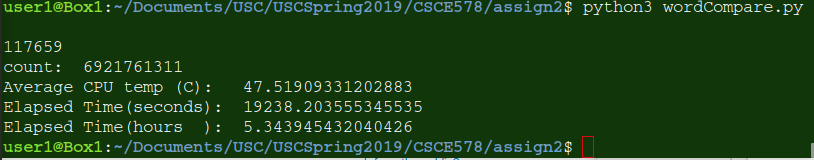
\includegraphics[width=\linewidth]{download.png}
  \caption{console output after running code}
\end{figure}
\par When the actual code was ran overnight all synonyms with a match of a bag intersection of over $70\%$ were printed out to a file. This low intersection requirement was chosen so that it would be possible to slowly increase the calibration until there was a low error rate. This results in a total of 31956 matches being found with a match of at least .7  After this, the list of outputted synonyms was checked and refined based on the intersection size between the words until a decent success rate was obtained. \\The results are shown below:
\begin{center}
 \begin{tabular}{||c | c||} 
 \hline
 Interstion Rate & Synonym Count \\ [0.5ex] 
 \hline\hline
$>$.7 & 31965 \\ 
 \hline
= .75 & 21742 \\
 \hline
$>$.75 & 7206 \\
 \hline
$>$.8 & 3026 \\
 \hline
$>$.9 & 1122 \\
 \hline
$>$.95 & 771 \\
 \hline
= 1 & 768 \\ [1ex] 
 \hline
\end{tabular}
\end{center}

Through this is it seen that the majority of words had an intersection between of less than .8, with an extreme majority of intersections being exactly .75. The most reasonable explanation for this is the fact that no words with a definition length of less than 4 was computed, and a large amount of definitions were exactly at length 4, this caused many fractions in the $\frac{1}{4}$,$\frac{2}{4}$,$\frac{3}{4}$ set with $\frac{3}{4}$, being .75.
\par Looking at the actual results it is possible to see that there is quite a decent range of correctness in the success rate of synonym matching, even in the higher intersection rates of over .9. A few examples of this includes terms such as "inside\_loop", and "outside\_loop", these terms are opposites in the fact that they are two different aviation maneuvers. However, the definitions with stop words included again are :
\\"a loop consisting of a climb followed by inverted flight followed by a dive that returns to horizontal flight"
\\"a loop consisting of a dive followed by inverted flight followed by a climb that returns to horizontal flight"
\\ These two definitions have a different meaning, however within a bag they use the exact same words, this causes the intersection rate to be 1, and them to be counted as synonyms even with the highest level of calibration.
\\ Another good example of this is with terms from baseball such as "single", "double", and  "triple". The definitions of these examples are:
\\"a base hit on which the batter stops safely at first base"
\\"a base hit on which the batter stops safely at second base"
\\"a base hit at which the batter stops safely at third base" 
\\As can be seen these are nearly identical definitions with just a single word different causing a set intersection of .83. 
\par This is quite a rampant issue that was encountered prominently throughout this project, overall there was a higher rate of these terms being matched than actual synonyms being matched. Because of this it is more fair to say that a list of interrelated terms was created, than a list of synonyms. Whenever words, such as baseball terms, minerals, States, aviation terms, and fish, were encountered, they would be grouped together because of the large set intersections that were found. This is not to say that there were no synonyms found, there were still terms like, "glaucomys" and "american\_flying\_squirrel", or "ketch" and "yawl". These terms are exact synonyms of each other and the program was able to find a few of these as well.
\par In the future, when this project is expanded, there would have to be quite a large change in the way that would cause words to be linked based on being synonyms. This will be quite a process as to how these will be differentiated, and in what way it will be determined if the words are synonyms.
\end{addmargin}
What each file is:
\begin{addmargin}[4em]{4em}
finalOut.txt - The output of all matches $>$.7\\
/dict/form.txt - The formatted dictionary in text file\\
/dict/stopless.txt - The dictionary without stop words\\
makedict.py - The creating of all the dictioanry files, from formatting the original dictionary to remove stop words\\
wordCompare.py - the comparison of all of the words\\
synonymSort.py - sorting words based off of their intersection value\\
\end{addmargin}




\end{document}
